\documentclass[10pt]{article}
\usepackage{amssymb}
\usepackage{amsmath}
\usepackage{mathdots}
\usepackage{color}
\usepackage{textcomp}
\usepackage[pdftex]{graphicx}
\usepackage{tikz}
\usepackage{enumerate}
\usepackage[margin=1in,footskip=0.25in]{geometry}
\newcommand{\mtrx}[1]{\begin{bmatrix}#1\end{bmatrix}}
\newcommand{\angles}[1]{\langle#1\rangle}
\newcommand{\floor}[1]{{\left\lfloor#1\right\rfloor}}
\let\oldemptyset\emptyset
\let\emptyset\varnothing
\let\union\cup
\let\intersect\cap
\begin{document}
% :r!./emit_deployment_diagram.ml
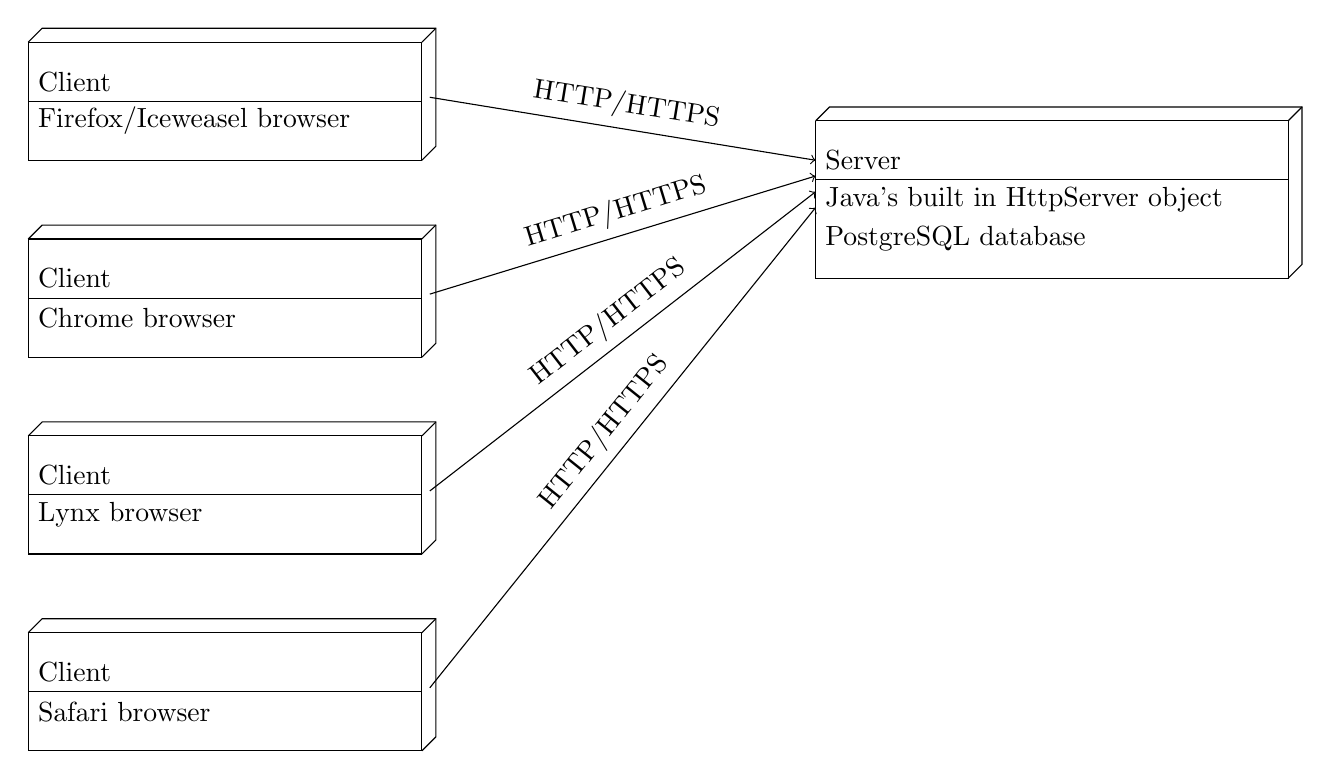
\begin{tikzpicture}
\draw[-, color=black] (0.000000, 0.000000) -- (5.000000, 0.000000) -- (5.000000, -1.500000) -- (0.000000, -1.500000) -- (0.000000, 0.000000);
\draw[-, color=black] (0.000000, 0.000000) -- (0.176777, 0.176777) -- (5.176777, 0.176777) -- (5.176777, -1.323223) -- (5.000000, -1.500000);
\draw[-, color=black] (5.000000, 0.000000) -- (5.176777, 0.176777);
\draw[color=black] (0.000000, -0.500000) node[right]{Client};
\draw[color=black] (0.000000, -1.000000) node[right]{Firefox/Iceweasel browser};
\draw[-, color=black] (0.000000, -0.750000) -- (5.000000, -0.750000);
\draw[-, color=black] (0.000000, -2.500000) -- (5.000000, -2.500000) -- (5.000000, -4.000000) -- (0.000000, -4.000000) -- (0.000000, -2.500000);
\draw[-, color=black] (0.000000, -2.500000) -- (0.176777, -2.323223) -- (5.176777, -2.323223) -- (5.176777, -3.823223) -- (5.000000, -4.000000);
\draw[-, color=black] (5.000000, -2.500000) -- (5.176777, -2.323223);
\draw[color=black] (0.000000, -3.000000) node[right]{Client};
\draw[color=black] (0.000000, -3.500000) node[right]{Chrome browser};
\draw[-, color=black] (0.000000, -3.250000) -- (5.000000, -3.250000);
\draw[-, color=black] (0.000000, -5.000000) -- (5.000000, -5.000000) -- (5.000000, -6.500000) -- (0.000000, -6.500000) -- (0.000000, -5.000000);
\draw[-, color=black] (0.000000, -5.000000) -- (0.176777, -4.823223) -- (5.176777, -4.823223) -- (5.176777, -6.323223) -- (5.000000, -6.500000);
\draw[-, color=black] (5.000000, -5.000000) -- (5.176777, -4.823223);
\draw[color=black] (0.000000, -5.500000) node[right]{Client};
\draw[color=black] (0.000000, -6.000000) node[right]{Lynx browser};
\draw[-, color=black] (0.000000, -5.750000) -- (5.000000, -5.750000);
\draw[-, color=black] (0.000000, -7.500000) -- (5.000000, -7.500000) -- (5.000000, -9.000000) -- (0.000000, -9.000000) -- (0.000000, -7.500000);
\draw[-, color=black] (0.000000, -7.500000) -- (0.176777, -7.323223) -- (5.176777, -7.323223) -- (5.176777, -8.823223) -- (5.000000, -9.000000);
\draw[-, color=black] (5.000000, -7.500000) -- (5.176777, -7.323223);
\draw[color=black] (0.000000, -8.000000) node[right]{Client};
\draw[color=black] (0.000000, -8.500000) node[right]{Safari browser};
\draw[-, color=black] (0.000000, -8.250000) -- (5.000000, -8.250000);
\draw[-, color=black] (10.000000, -1.000000) -- (16.000000, -1.000000) -- (16.000000, -3.000000) -- (10.000000, -3.000000) -- (10.000000, -1.000000);
\draw[-, color=black] (10.000000, -1.000000) -- (10.176777, -0.823223) -- (16.176777, -0.823223) -- (16.176777, -2.823223) -- (16.000000, -3.000000);
\draw[-, color=black] (16.000000, -1.000000) -- (16.176777, -0.823223);
\draw[color=black] (10.000000, -1.500000) node[right]{Server};
\draw[color=black] (10.000000, -2.000000) node[right]{Java's built in HttpServer object};
\draw[color=black] (10.000000, -2.500000) node[right]{PostgreSQL database};
\draw[-, color=black] (10.000000, -1.750000) -- (16.000000, -1.750000);
\draw[->] (5.100000, -0.700000) -- node[above, rotate=-9.272602]{HTTP/HTTPS} (10.000000, -1.500000);
\draw[->] (5.100000, -3.200000) -- node[above, rotate=17.020526]{HTTP/HTTPS} (10.000000, -1.700000);
\draw[->] (5.100000, -5.700000) -- node[above, rotate=37.793943]{HTTP/HTTPS} (10.000000, -1.900000);
\draw[->] (5.100000, -8.200000) -- node[above, rotate=51.225829]{HTTP/HTTPS} (10.000000, -2.100000);
\end{tikzpicture}
\end{document}
